\documentclass[UTF8,12pt]{ctexart}
\title{有理数 - Rational Number}
\author{作者:K}
\date{最后更新:\today}
\usepackage{amsmath}
\usepackage{graphicx}
\usepackage{geometry}
\usepackage{setspace}
\onehalfspacing
\geometry{papersize={25cm,25cm}}
\geometry{left=3cm,right=3cm,top=3cm,bottom=4cm}

\usepackage[section]{placeins}

\usepackage{fontspec}

%\setmainfont{Times New Roman}
%\setsansfont{Myriad Pro}
%\setmonofont{Courier Std}

%\setCJKmainfont[BoldFont={方正小标宋_GBK},ItalicFont={方正楷体_GBK},BoldItalicFont={方正仿宋_GBK}]{方正书宋_GBK}
\setCJKmainfont{Microsoft YaHei}
\setCJKsansfont{SimHei}
\setCJKmonofont{DengXian}

\addtolength{\parskip}{1.2em}   %段间距

\begin{document}
\maketitle
%\tableofcontents
\newpage

\section{有理数}
有理数的概念:整数和分数统称为有理数(Rational Number)。

我们可以把有理数看做分数。因为整数也可以表示成分数,所以有理数都可以写成 $ \dfrac{p}{q} $ 的形式。

我们可以把有理数看做无限循环的小数。分数可以化成有限小数和无限循环的小数,只要我们把有限小数看做是循环节为0的无限循环小数,那么分数可以看做是无限循环小数。那么有理数就都可以看做是无限循环小数。

\begin{figure}[htb]
\centering

\includegraphics[width = .5\textwidth]{decimal.jpg}
\caption{小数与分数}
\label{fig:decimal}
\end{figure}

\newpage
\section{数轴、相反数和绝对值} 

数轴(Number Axis)三要素:原点,正方向,单位长度。

\begin{figure}[htb]
\centering
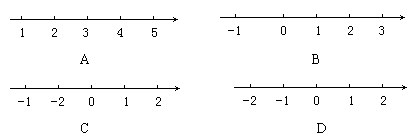
\includegraphics[width = .85\textwidth]{number-axis.png}
\caption{哪个数轴画得对?}
\label{fig:number-axis}
\end{figure}

相反数(Opposite Number):只有符号不同的一对数。我们把数a的相反数记作-a。表示互为相反数的两个数的点,在数轴上分别位于原点的两侧,并且与原点的距离相等。即关于原点对称。

绝对值(Absolute Value):数轴上的点到原点的距离,它一定是一个非负数。正数的绝对值是它本身,负数的绝对值是它的相反数,0的绝对值是0。互为相反数的两个数的绝对值相等。

\subsection{问题}
1.\quad $ -|-3.8| = ? $

2.\quad 数轴上表示绝对值等于3.5的数的点有几个?分别是多少?

\newpage
\section{有理数大小的比较}

在以向右为正方向的数轴上,右边的点表示的数比左边的点表示的数大。

看图\ref{fig:number-comparison},思考怎么比较两个负数的大小。

\begin{figure}[htb]
\centering
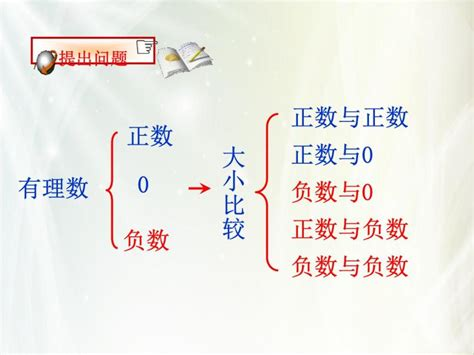
\includegraphics[width = .55\textwidth]{number-comparison.jpg}
\caption{数的比较}
\label{fig:number-comparison}
\end{figure}

两个负数,绝对值大的反而小。

\subsection{问题}
1. \quad 比较大小:$ -\dfrac{3}{10} $ 与 $ -|-\dfrac{2}{5}| $

\newpage
\section{加减法}

加法(Addition)的一般规则:
\begin{figure}[htb]
\centering

\includegraphics[width = .55\textwidth]{addition.png}
\caption{加法}
\label{fig:addtion}
\end{figure}

减法(Subtraction)的一般规则(减法化成加法做):
\begin{figure}[htb]
\centering
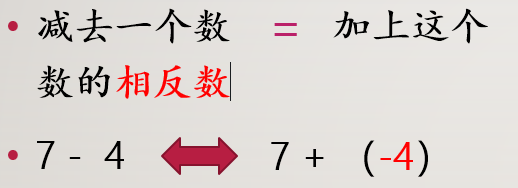
\includegraphics[width = .55\textwidth]{subtraction.png}
\caption{减法}
\label{fig:subtraction}
\end{figure}

加减混合运算注意事项:因为减法不像加法那样具有交换律(Commutative law)、结合律(Associative law),因此不能对减法进行交换结合。即不要乱动减法,只能在加法间运用交换律结合律。除非你将减法化成加法。

“去掉前面带有减号(或负号)的括号”的法则:括号前面是“-”号时,把括号连同它前边的“-”号都去掉,括号里各数都变号。比如 $ -(-7) = 7 $,$ -(1+2) = -1-2 $,$ -(3-1+2) = -3+1-2 $ 。可以通过乘以-1的分配律来理解。相反,如果括号前面是“+”号,同样将括号连同它前边的“+”去掉,但是括号里各数的符号不变。

\begin{figure}[htb]
\centering
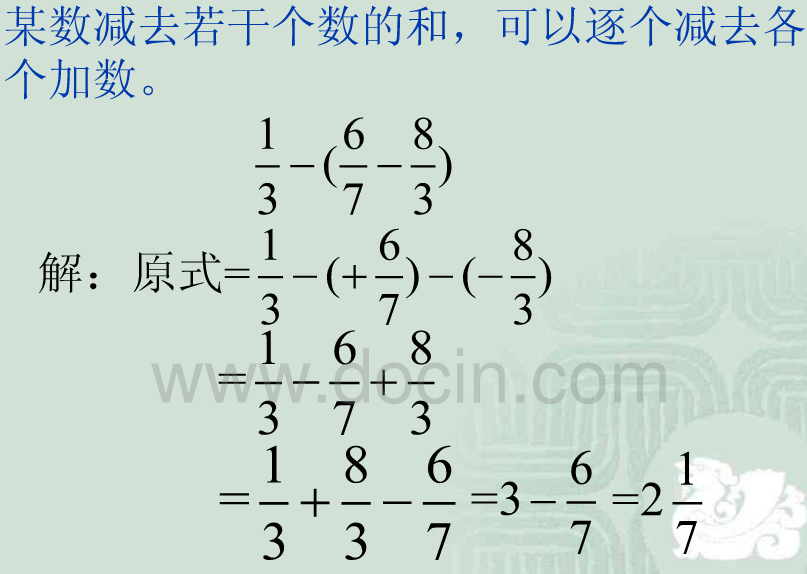
\includegraphics[width = .55\textwidth]{quit-bracket.png}
\caption{去括号}
\label{fig:quit-bracket}
\end{figure}

\subsection{问题}
1. \quad -40 - (+28) + (-19) - 24 - 23

2. \quad $ 15 - (+\dfrac{5}{6}+\dfrac{3}{7}) + (-\dfrac{1}{6}-\dfrac{4}{7}) $

\newpage
\section{乘除法}
乘法(Multiplication)的一般规则:

\begin{figure}[htb]
\centering

\includegraphics[width = .75\textwidth]{multiplication.png}
\caption{两个数的乘法}
\label{fig:multiplication}
\end{figure}

两数相乘,同号得正,异号得负,绝对值相乘。

多数相乘,奇负偶正,绝对值相乘。

如果两个数的乘积等于1,我们把其中一个数叫做另一个数的倒数(reciprocal),也称它们互为倒数。

乘法和加法类似,都有交换律、结合律。乘法还有对加法的分配律(Distributive law)。

\newpage
除法(Division)法则:
\begin{figure}[htb]
\centering

\includegraphics[width = .5\textwidth]{division.png}
\caption{除法}
\label{fig:division}
\end{figure}

\subsection{问题}
1. \quad -0.25的倒数是多少?

2. \quad $ (-4)\div(-8)\times\dfrac{1}{8} $

3. \quad 如果两个有理数的积是正的,那么这两个因数的符号是什么关系。

4. \quad $ (-1155) \div [(-11) \times (+3) \times (-5)] $

5. \quad $ -81 \div \dfrac{1}{3} - \dfrac{1}{3} \div (-\dfrac{1}{9}) $

\end{document}